\section{Motivation}

\begin{frame}{Why build Language Models?}
\begin{itemize}
    \item Originally intended to solve the task of language modelling.
\end{itemize}

\begin{block}{Language Modelling - informal but legit definition}<+->
% is the task of defining a conditional probability distribution over each token in a sequence conditioned on the previous observations. Consider a sequence of arbitrary length $T$, $\{x_1, x_2, \dotsc, x_{t-1}, x_t, x_{t+1},  \dotsc, x_T \}$ and let $x_t$ denote the $t$th token and $x_{1}^{t-1}$ express the sequence of tokens from $1, \dotsc, t-1$. Then then goal of language modelling is to predict the probability distribution of $x_t$ conditioned on $x_1^{t-1}$, i.e., $p(x_t | x_1^{t-1})$.
Language Modelling is the task of predicting the next token conditioned on some previous context
\end{block}
\begin{itemize}
    \item Currently utilised to create contextual word representations employed on a myriad of downstream tasks.
\end{itemize}
\begin{block}{Language Model (LM) usage in Natural Language Processing (NLP)}<+->
	LMs are utilised ubiquitously for NLP tasks including language modelling, speech recognition and question answering.
\end{block}
\end{frame}

% Language model examples (use-cases)
\begin{frame}{Language Model Use-case I: Language modelling}
Consider the context,
    \begin{equation*}
    p(X) = p(x|\textsf{the Ballmer peak is a}).
\end{equation*}
Here we would like the distribution over $x$ to look something like:
\begin{equation*}
    p(X) =  
    \begin{cases}
        0.37, & x=\textsf{myth} \\
        0.45, & x=\textsf{fictional} \\
        0.02, & x=\textsf{factual} \\
        0.16, & x \in V \backslash \{\textsf{myth}, \textsf{fictional}, \textsf{factual}\}
    \end{cases}
\end{equation*}
\end{frame}

% speech recognition
\begin{frame}{Language Model Use-case II: Speech Recognition}
    
    \begin{figure}
        \centering
        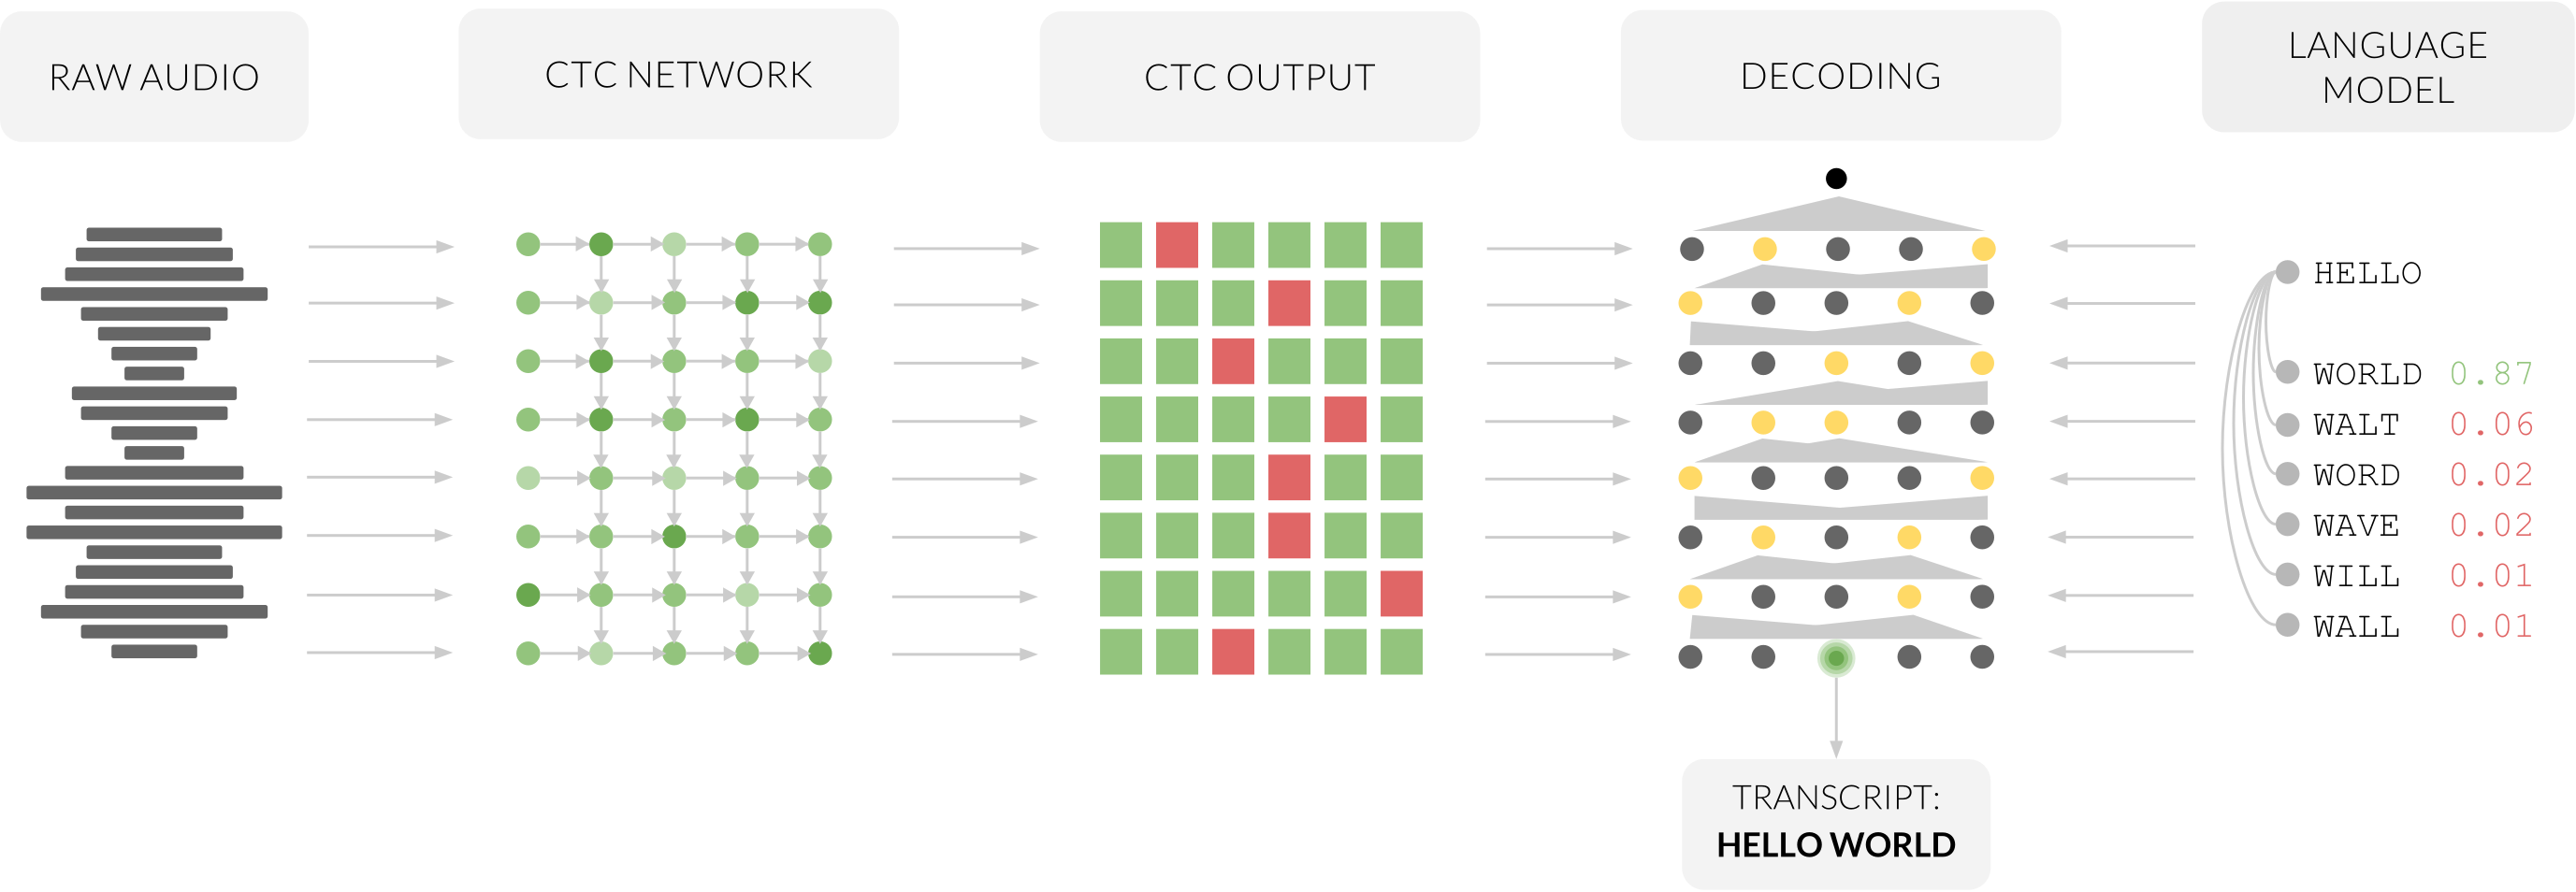
\includegraphics[width=\textwidth]{graphics/use-cases/ctc_network.png}
    \end{figure}
    {\footnotesize Courtesy of Corti.ai}
\end{frame}

% Question Answering - Reading Comprehension
\begin{frame}{Language Model Use-case III: Question-Answering (QA)}
    \begin{figure}
        \centering
        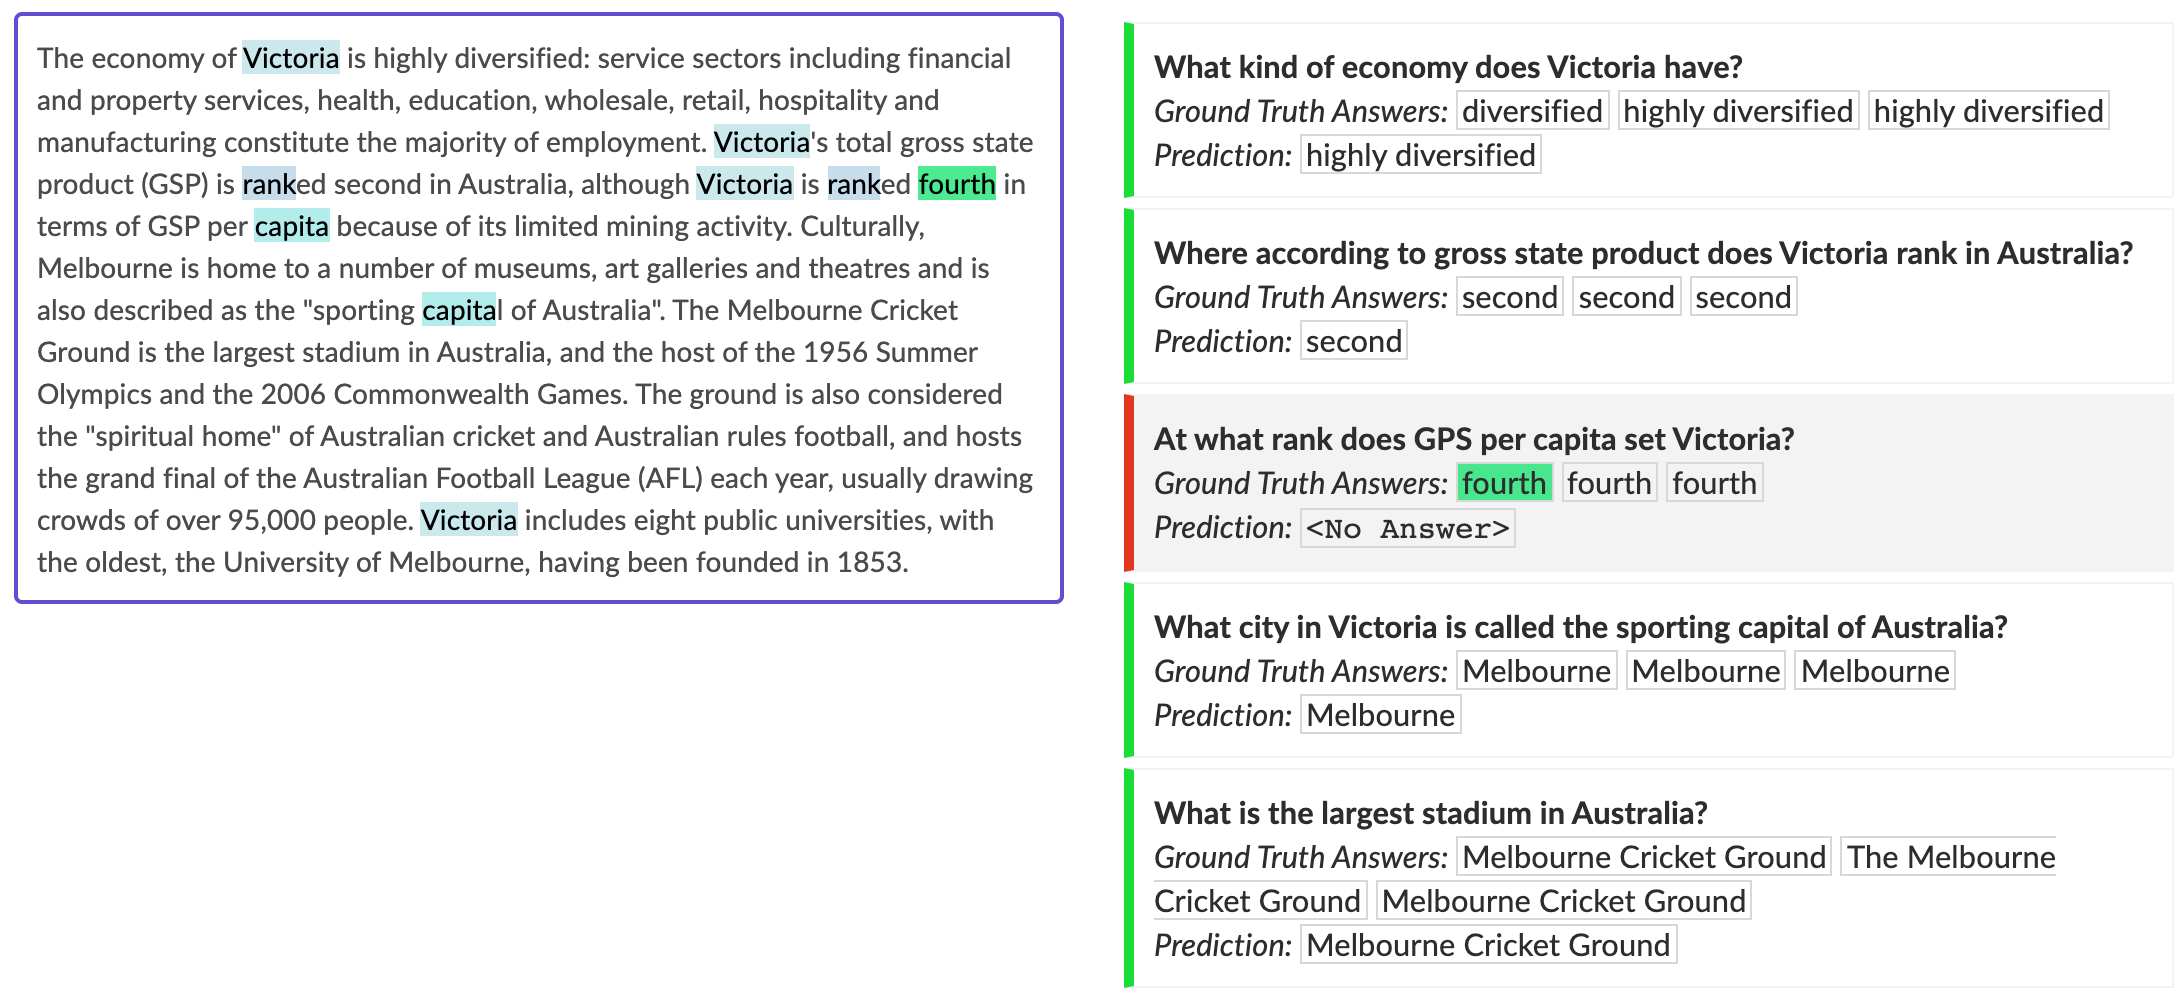
\includegraphics[height=0.8\textheight]{graphics/use-cases/question-answering.png}
    \end{figure}
    {\footnotesize Example from the SQuAD v2.0 dataset}
\end{frame}

% Model size Evolution
\begin{frame}{Visualising the Research Trends - Courtesy of HuggingFace}

    \begin{figure}
        \centering
        \begin{tikzpicture}
        \begin{scope}[zlevel=main]
            \node[anchor=south,inner sep=4pt,minimum width=2cm, minimum height=1cm ,outer sep=0pt,rounded corners=4pt,fill=DTU_red,draw=black!70, text=white, rotate=33] at (0,1.6) {YES. Indeed a terrifying curve!};
            \node[text width=1.5cm, align=center] (T5) at (7.3, 3.5) {\footnotesize T5 \,\, 11300 Google};
            \node[dot, draw=DTU_blue, fill=DTU_blue] at (6.8, 3.9) {};
            \node[rotate=45, black!50] at (6.85, -2.7) {\tiny October 2019};
        \end{scope}
        \begin{scope}[zlevel=-1]
        \node at (0,0) {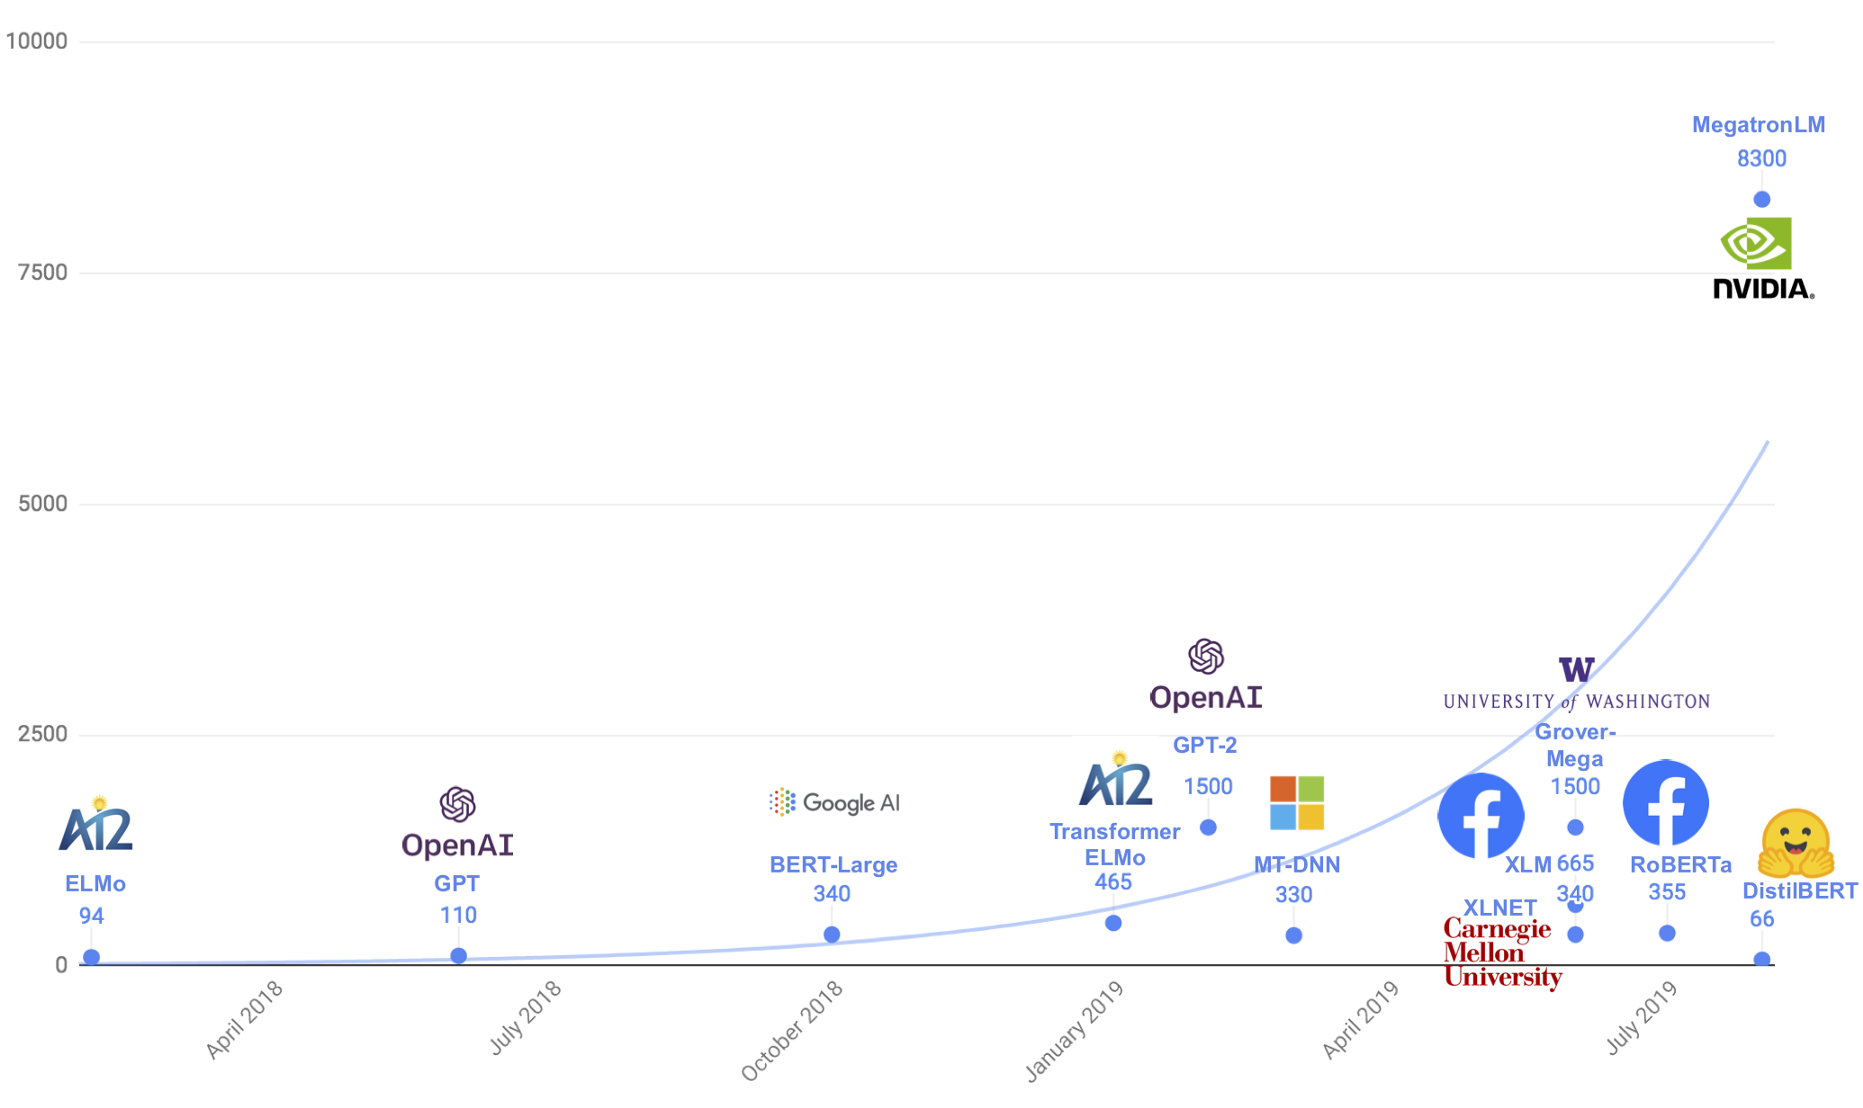
\includegraphics[width=0.8\textwidth]{graphics/auxillary/model_complexity.png}};
        \end{scope}
        \end{tikzpicture}
    \end{figure}
\end{frame}


% Current Research Trends
\begin{frame}{(Some of the) Current Research Directions} 
\begin{enumerate}
    \item \textbf{Ramping up the number of parameters }
    \begin{itemize}
        \item In 2018 \cite{Devlin2018BERT:Understanding} published BERT-large with 340M tunable parameters. 
        \item The current leader on the General Language Understanding Evaluation (GLUE) and SuperGLUE benchmarks is T5 with unfathomable 11B tunable parameters \cite{Raffel2019ExploringTransformer}. 
    \end{itemize}
    \item \textbf{Learning more effectively}
    \begin{itemize}
        \item Parameter initialisation techniques \cite{Frankle2018TheNetworks, Yu2019PlayingNLP}
        \item Knowledge Distillation \cite{Sanh2019DistilBERTLighter}
        \item \textcolor{DTU_red}{\textbf{Infusing external knowledge}} \cite{Logan2019BaracksModeling, Hayashi2019LatentModels, Peters2019KnowledgeRepresentations}
    \end{itemize}
    \item \textbf{Data augmentation}
    \begin{itemize}
        \item Varying the input at inference to make the model more robust using ensemble predictions \cite{Jiang2019HowKnow}
        \item Replacing semantically similar words \cite{Wang2015ThatsTweets}
        \item Generating new questions in visual question answering \cite{Kafle2017DataAnswering}
    \end{itemize}
\end{enumerate}
\end{frame}


% External Knowledge Representations Intermezzo
\begin{frame}{Intermezzo: External Knowledge Representations }
    \begin{columns}
    \begin{column}[T]{0.5\textwidth}
    {\color{DTU_blue}\rule{\linewidth}{4pt}
    Knowledge Base (KB)  \hfill\rule{\linewidth}{4pt}}
    \begin{figure}
        \centering
        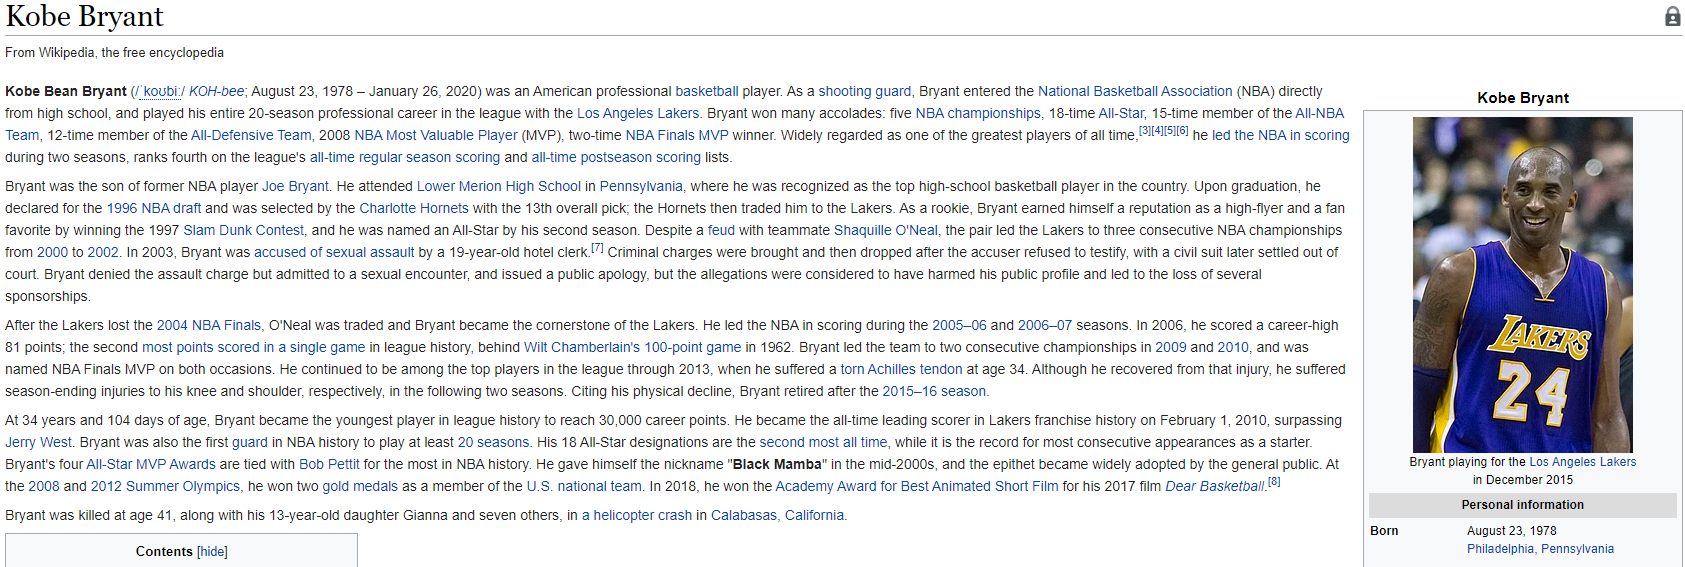
\includegraphics[height=2.2cm]{graphics/auxillary/KB_example.PNG}
    \end{figure}
    \vfill
    \begin{center}
        $\downarrow$ \\
        $e_{\mathrm{kobe}} \in R^{E_{\mathrm{arb.}}}$
    \end{center}
    \end{column}
    \begin{column}[T]{0.5\textwidth}
    {\color{DTU_orange}\rule{\linewidth}{4pt}
    Knowledge Graph (KG) \hfill\rule{\linewidth}{4pt}}
    \begin{figure}
        \centering
        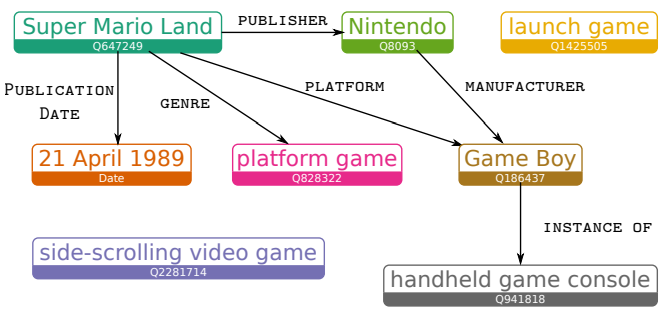
\includegraphics[height=2.2cm]{graphics/auxillary/KG_example.PNG}
    \end{figure}
    \vfill
    \begin{center}
        $\downarrow$ \\
        $e_{\mathrm{SML}} \in R^{E_{\mathrm{arb.}}}$ \\
        $\vdots$ 
    \end{center}
    \end{column}
    \end{columns}
\end{frame}

% Symbiosis between LM anad 
\begin{frame}{Symbiosis between LMs and KGs}
\begin{columns}
\begin{column}[T]{0.5\textwidth}<+->
\textbf{Language Models are}
    \begin{itemize}
        \item factually inconsistent,
        \item difficult to interpret in terms of understanding their decision-making,
        \item typically not able to cope well with real-world entities and rarely occurring words,
        \item to a moderate extent context-aware looking at the current state-of-the-art.
    \end{itemize}
\end{column}
\begin{column}[T]{0.5\textwidth}\onslide<+->
\textbf{Knowledge Graphs are}
    \begin{itemize}
        \item factually consistent (\textit{given the knowledge graphs are updated}),
        \item interpretable in the sense that we know the relations between entities,
        \item commonly entailing a lot of real-world entities falling into the category of rare words for language models,
        \item not a human-friendly interface in many cases.
    \end{itemize}
\end{column}
\end{columns}
\vspace{5pt}
\end{frame}

\frame{
    \frametitle{Idea - A synergistic relationship between LMs and KGs}
\begin{block}{Goal}<+->
  Establish a synergistic relationship between LMs and KGs by dynamically allowing LMs to augment their knowledge drawing upon relevant information entailed by a KGs.
\end{block}
\begin{center}
    \textcolor{DTU_red}{\textbf{\textit{"How?"} one might ponder}}
\end{center}
\begin{columns}
\begin{column}[T]{0.5\textwidth}<+->
    {\color{DTU_red}\rule{\linewidth}{3pt}
    Task-specific methods \hfill\rule{\textwidth}{3pt}}
    \begin{itemize}
        \item Commonly joint learn task-specific and KG related objectives
        \item After which we at inference can marginalise over entity information
    \end{itemize}
\end{column}
\begin{column}[T]{0.5\textwidth}<+->
    {\color{DTU_red}\rule{\linewidth}{3pt}
    General-purpose methods \hfill\rule{\textwidth}{3pt}}
    \begin{itemize}
        \item Task-agnostic augmentation
        \item Draws indirectly from external entities
    \end{itemize}
\end{column}
\end{columns}
}